% Permission is granted to copy, distribute and/or modify this document
% under the terms of the GNU Free Documentation License, Version 1.3
% or any later version published by the Free Software Foundation;
% with no Invariant Sections, no Front-Cover Texts, and no Back-Cover Texts.
% A copy of the license is included in the section entitled "GNU
% Free Documentation License".
%
% Authors:
% Caner Candan <caner@candan.fr>, http://caner.candan.fr

\documentclass{beamer}
\usepackage[french]{my_package}

\title[Outil de profiling \emph{myproof}]{Présentation de \emph{myproof}}

\begin{document}

\begin{frame}
  \titlepage
\end{frame}

\begin{frame}{Features}
\begin{figure}[here]
  \centering
  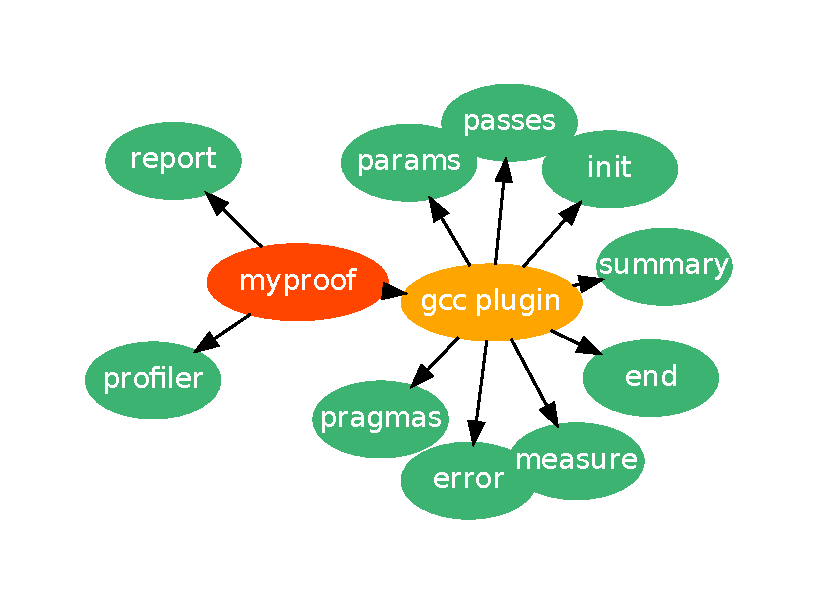
\includegraphics[scale=0.7]{images/schema.pdf}
  \caption{Hierarchy of features}
\end{figure}
\end{frame}

\begin{frame}{Introduction}
  \begin{itemize}
  \item Logiciel de profiling
  \item Interface Modulable
  \item Gestion des pragmas
  \item Instrumentation statique
  \item Instrumentation dynamique
  \item Analyse et visualisation des résultats
  \item Et le multithreading ?
  \end{itemize}
\end{frame}

\begin{frame}{Directives pragma}
 \begin{itemize}
  \item Souci de modularité
  \item 2 styles de déclarations
    \begin{itemize}
    \item pragma instrumente foo
    \item pragma instrumente (fct1, fct2)
    \end{itemize}
  \item Gestion d'erreur
  \end{itemize}
 \end{frame}

\begin{frame}{Instrumentation statique}
  \begin{itemize}
  \item Instrumentation ``statique'' $\rightarrow$ Compilation
  \item Inspection des accès mémoire (load/store)
  \item On cherche à détecter les blocs de base ainsi que les boucles
  \item 2 passes concernées: ``pass\_loop'' et ``pass\_bb''
  \item Parcours des blocs de base
  \item Représentation GIMPLE
  \item Affectation (GIMPLE\_ASSIGN) ?
  \item Analyse des opérandes
  \item Utilisation de la passe de référence "parloops" ainsi que des options d'optimisation "-O1" ou "-O2"
  \item Permet de générer un graphe CFG
  \end{itemize}
\end{frame}

\begin{frame}{Instrumentation dynamique}
  \begin{itemize}
  \item Le pragma permet d'enregistrer les fonctions à instrumenter
  \item Parcours des blocs de base d'entrée et de sortie des fonctions à l'aide d'une passe d'instrumentation
  \item On utilise une librairie ``measure'' contenant ``myproof\_measure\_start(fname)'' et ``myproof\_measure\_stop''
  \item Mesure avec l'instruction assembleur RDTSC
  \end{itemize}
 \end{frame}

\begin{frame}{Analyse des instrumentations}
  \begin{itemize}
  \item Parsing des fichiers de sortie (LEX et YACC)
  \item Profilage inclusif $\rightarrow$ profilage exclusif ? Arbre n-aire
  \item Détection des imbrications entre fonctions
  \item Gestion des instances $\rightarrow$ comparaison des temps d'exécution
  \item Corrélation entre instrumentations statique et dynamique
  \item Calcul des latences de load et store ? Non
  \item Graphe d'appel des fonctions
  \end{itemize}
\end{frame}

\begin{frame}{Et le multithreading ?}
  \begin{itemize}
  \item Exécution multithreadée $\rightarrow$ écriture concurrente sur les prises de mesure
  \item Utilisation des mutex accès exclusif aux données
  \item Sémaphores POSIX $\rightarrow$ synchronisation des actions entre processus
  \item Mot clé ``\_thread''
  \end{itemize}
\end{frame}

\end{document}
